\documentclass[ALICE,manyauthors]{ALICE_analysis_notes}
%\documentclass[ALICE,manyauthors]{ALICE_scientific_notes}
%
%\newcommand{\jpsi}{\rm J/$\psi$}
%\newcommand{\psip}{$\psi^\prime$}
%\newcommand{\jpsiDY}{\rm J/$\psi$\,/\,DY}
%\newcommand{\dd}{\mathrm{d}}
%\newcommand{\chic}{$\chi_{\rm c}$}
%\newcommand{\ezdc}{$E_{\rm ZDC}$}
%\newcommand{\red}{\textcolor{red}}
%\newcommand{\blue}{\textcolor{blue}}
\newcommand{\slfrac}[2]{\left.#1\right/#2}
\newcommand{\sNN}{$\sqrt{s_{\mathrm{NN}}} = $\xspace}
\newcommand{\pip}{$\pi^{+}$\xspace}
\newcommand{\pim}{$\pi^{-}$\xspace}
\newcommand{\kap}{K$^{+}$\xspace}
\newcommand{\kam}{K$^{-}$\xspace}
\newcommand{\pbar}{$\rm\overline{p}$\xspace}
\newcommand{\degree}{$^{\rm o}$\xspace}
\newcommand{\s}{$\sqrt{s}=$\xspace}
\newcommand{\pt}{\ensuremath{p_{\rm T}}\xspace}
\newcommand{\dedx}{d$E$/d$x$\xspace}
\newcommand{\dndy}{d$N$/d$y$\xspace}
\newcommand{\dndydpt}{${\rm d}^2N/({\rm d}y {\rm d}p_{\rm T})$\xspace}
\newcommand{\pp}{pp\xspace}
\newcommand{\pbpb}{Pb--Pb\xspace}
\newcommand{\raa}{$R_{\mathrm{AA}}$\xspace}
\newcommand{\Dstar}{D$^{*+}$\xspace}
\newcommand{\Dzero}{D$^0$\xspace}
\newcommand{\Dplus}{D$^+$\xspace}
\newcommand{\Dsubs}{D$^+_{\mathrm{s}}$\xspace}
\newcommand{\MeV}{{\rm MeV}}
\newcommand{\GeV}{{\rm GeV}}
\newcommand{\TeV}{{\rm TeV}}
\newcommand{\TAA}{T_{\mathrm{AA}}}
\newcommand{\RAA}{R_{\mathrm{AA}}}
\newcommand{\mum}{\mu{\rm m}}
\newcommand{\de}{{\rm d}}
\usepackage{rotating}
\usepackage{graphicx}
\usepackage{lineno}
%
\begin{document}%
%%%%%%%%%%%%% ptdr definitions %%%%%%%%%%%%%%%%%%%%%
%
%%%%%%%%%%%%%%%  Title page %%%%%%%%%%%%%%%%%%%%%%%%
%
\begin{titlepage}
%
\PHnumber{ALICE-ANA-2022-xxx} 
\PHdate{\today}
%
%%% Put your own title + short title here:
\title{Prompt \Dstar mesons production in pp collisions at \s 13 TeV}
\ShortTitle{\Dstar meson production in pp collisions at \s 13 TeV}   % appears on right page headers
%
\author{Syaefudin Jaelani$^{1}$}
\author{
1. Indonesian Institute of Sciences
}
\author{Email: syaefudin.jaelani@cern.ch}
%
\ShortAuthor{ALICE Analysis Note 2019}      % appears on left page headers, do not change
%
%\linenumbers
\begin{abstract}
The production of prompt \Dstar mesons and their anti-particles was measured using the 2016, 2017 and 2018 data samples of pp collisions at \s 13 TeV collected by the ALICE collaboration. The production cross-sections are measured at mid-rapidity as a function of \pt, in the range 1 $<$ \pt $<$ 50 GeV/$c$.

%The \pt-differential production yields at central rapidity ($|y|<$0.5), in the range 1 $<$ \pt $<$ 50 GeV/$c$, were used to evaluate the nuclear modification factor \raa with respect to the pp reference at \s 5 TeV measured by the ALICE Collaboration \cite{Acharya:2019mgn}. The calculation is performed in two centrality classes, 0--10$\%$ and 30--50$\%$. The ratios of \Dzero/\Dsubs, \Dplus/\Dsubs and \Dstar/\Dsubs are also studied in order to investigate a possible different suppression of charm and strange mesons. This might bring insight in the hadronization mechanism which can play a role in charm mesons formation.  
\end{abstract}
\end{titlepage}
%
%\input{alice_mynote.tex}               %%%%%%%%%%% put the body of the article here
\tableofcontents
\cleardoublepage
\input{intro.tex}
%\clearpage
\section{D meson selection}
The \Dstar meson and their anti-particles was reconstructed in the central rapidity region by exploiting their charged hadronic decay channels: \Dstar $\rightarrow$ \Dzero$\pi^{+}$ (with B.R. = 67.7 $\pm$ 0.5$\%$), while the \Dzero meson decay into $K^-$ and $\pi^{+}$ with branching ratio (3.93$\pm$0.04)\%. The \Dstar decay proceeds via strong interaction, thus making impossible the secondary vertex reconstruction. The analysis exploits topological selections on the \Dzero,  together with the sharp peak in the difference between the invariant mass of the three final state hadrons and that of the two \Dzero decay prongs. Since the mass difference $\Delta m = m_{\rm D^{\ast +}} - m_{\rm D^0} \approx 145.4$ MeV/$c$ is only slightly larger than the charged pion mass. For low \pt \Dstar mesons the produced pion has typically low momentum and is referred to here as a soft pion.


%In this case the selection is applied to the decay topology of the daughter \Dzero. The selection of \Dzero candidates is based on the reconstruction of the displaced secondary vertex topologies, with a typical separation of $\sim$ 100$\mu$m from the interaction point. The \Dstar meson raw yields are extracted from the invariant mass distributions obtained from the analysis of fully reconstructed decay topologies displaced with respect to the primary vertex.

\subsection{Single track selections}
\label{sec:single_track}

The \Dstar candidates were formed by combining \Dzero candidates with soft pion $\pi^{+}$ tracks having $|\eta| <$ 0.8 and \pt $>$ 0.3 GeV/$c$, also satisfying the kITSrefit and kTPCrefit conditions. Moreover, for all the tracks, a minimum number of 70 crossed rows in the TPC together with a crossed rows over findable clusters ratio of 0.8 was required, and $\chi^2$/$ndf <$ 2 in the TPC. A cut on the transverse impact parameter $d_0$ was applied for tracks with \pt $<$ 2 GeV/$c$, requiring $d_0 >$ 50 $\mu$m. These selections were meant to limit the CPU time needed to perform the track combinatorics when creating the AODs with the D meson candidates. Furthermore, the \Dstar soft pions were selected requiring at least one associated hit in either of the two SPD layers.
% at least 70 out of 159 crossed TPC pad rows
% SetMinNCrossedRowsTPC(70)
% SetMinRatioCrossedRowsOverFindableClustersTPC(0.8)
% Moreover, for all the tracks, a minimum number of 70 crossed rows in the TPC together with a crossed rows over findable clusters ratio of 0.8 was required. 


  
  
%Secondary vertices of \Dzero and \Dplus meson candidates were constructed using tracks having $|\eta| <$ 0.8, \pt $>$ 0.5 GeV/$c$ and satisfying the kITSrefit and kTPCrefit conditions. Moreover, for all the tracks, a minimum number of 70 crossed rows in the TPC together with a crossed rows over findable clusters ratio of 0.8 was required. A cut on the transverse impact parameter $d_0$ was applied for tracks with \pt $<$ 2 GeV/$c$, requiring $d_0 >$ 50 $\mu$m. These selections were meant to limit the CPU time needed to perform the track combinatorics when creating the AODs with the D meson candidates. Furthermore, all tracks, including the \Dstar soft pion, were selected requiring at least 70 (out of a maximum of 159) associated space points and $\chi^2$/$ndf <$ 2 in the TPC, and at least one associated hit in either of the two SPD layers.

\subsection{Topological and kinematic selections}
%The yield extraction was performed using a particle selection strategy that has high efficiency and high statistical significance for the \Dstar meson signal.
%The same topological variables as in previous \Dstar -meson analyses were used in this analysis.

The \Dstar signal extraction is based on topological selections of displaced secondary vertices from \Dzero -meson candidates. For a detailed explanation of the procedure refer to \cite{Adam:2015sza}. The topological and kinematic cuts used to select the \Dstar -meson signal in pp collisions at \s 13 TeV are reported in Table~\ref{tab:CutDstar} and ~\ref{tab:CutDstar2}.

%The same topological and kinematic variables used for the analyses with the 2015 \pbpb data sample are reported. In particular, we recall the introduction of a topological variable introduced in \cite{Bruna:2016mgn} :

% the normalized impact parameter (IP) resolution. It is defined as the difference between the expected impact parameter value $d^{exp}_{0,T,\phi} \approx L_{xy} \cdot sin(\theta_{xy})$, where $L_{xy}$ is the decay length on $xy$ plane and $\theta_{xy}$ is the angle between the reconstructed D meson and the charged particle on $xy$ plane, and the reconstructed one $d^{reco}_{0,T,\phi}$. This difference is then normalized by the square root of their respective uncertainties summed in quadrature. A selection based on this variable can reduce the feed-down D-meson efficiency while keeping higher that of prompt D mesons. The projections of the variables in the $xy$ plane are instead justified by the improving of the impact parameter resolution with respect to $z$-direction. More details on this variable can be found in \cite{Bruna:2016mgn}.

%In addition, \Dsubs candidates were selected by requiring that one of the two pairs of oppositely-charged tracks had an invariant mass compatible with the PDG world average for the $\phi$ mass (1.019 GeV/$c^2$). 
%In order to further suppress the combinatorial background, the angles $\theta^{*}(\pi)$ and $\theta^{'}$(K) were exploited. 
%The first one is the angle between the pion in the KK$\pi$ rest frame and the KK$\pi$ flight line, which is defined by the positions of the primary and secondary vertices in the laboratory frame, and the second one is the angle between one of the two kaons and the pions in the KK rest frame.
%In order to further suppress the combinatorial background, the angle $\theta^{'}$(K) was exploited. This is the angle between one of the two kaons and the pions in the KK rest frame.


\begin{table}[h!]
  \begin{center}
    \caption{Selections used for the \Dstar -meson in the transverse momentum intervals 1$<$\pt$<$6.5 GeV/$c$.}  
    \label{tab:CutDstar}
    \resizebox{\linewidth}{!}{\begin{tabular}{|c|c|c|c|c|c|c|c|c|c|c|c|c|}
    \hline
      \pt (GeV/$c$) variable & [1-1.5] & [1.5-2] & [2-2.5] & [2.5-3] & [3-3.5] & [3.5-4] & [4-4.5] & [4.5-5] & [5-5.5] & [5.5-6] & [6-6.5] \\
      \hline
      \hline
      $\Delta M_{\rm D^0}$ (GeV)  & 0.021 & 0.032 & 0.035 & 0.035 & 0.038 & 0.038 & 0.038 & 0.042 & 0.042 & 0.045 & 0.049\\
      \hline
      DCA (cm) & 0.022 & 0.038 & 0.03 & 0.03 & 0.03 & 0.03 & 0.042 & 0.042 & 0.05 & 0.05 &  0.1 \\
      \hline
      $Cos(\theta^*)$ & 0.9 & 0.9 & 0.8 & 0.8 & 0.8 & 0.8 & 0.9 & 0.9 & 1.0 & 1.0 & 1.0  \\
      \hline
      \pt($K$) (GeV/$c$) & 0.4 &  0.4 & 0.9 & 0.9 & 0.9 & 1.0 & 1.0 & 1.0 & 1.0 & 1.0 & 1.0 \\
      \hline
      \pt($\pi$) (GeV/$c$) & 0.4 &  0.4 & 0.9 & 0.9 & 0.9 & 1.0 & 1.0 & 1.0 & 1.0 & 1.0 & 1.0 \\
      \hline
      $d_{0,K}$ (cm) & 0.1 & 0.1 & 0.1 & 0.1 & 0.1 & 0.1 & 0.1 & 0.1 & 0.1 & 0.1 & 0.1\\
	  \hline
	  $d_{0,\pi}$(cm)& 0.1 & 0.1 & 0.1 & 0.1 & 0.1 & 0.1 & 0.1 & 0.1 &0.1 &0.1 & 0.1 \\
	  \hline
	  $d_{0,K} \times d_{0,\pi}$ (10$^{-3}$) (cm$^2$) & -0.00025   &-0.00025  &  -0.00019& -0.00019 & -0.000144 &-0.000144  & -2.8 $\times 10^{-5}$ &-2.8 $\times 10^{-5}$  & 5.5 $\times 10^{-5}$ & 5.5 $\times 10^{-5}$ &0.0001 \\
	  \hline
	  $Cos(\theta_{point})$ & 0.8 & 0.8 & 0.9  & 0.9 & 0.89 & 0.89 & 0.81 & 0.81 & 0.79 & 0.79 & 0.7  \\
	  \hline
	  Inv. mass half width of \Dstar (GeV) & 0.3 & 0.3 & 0.3 & 0.3 & 0.3 & 0.3 & 0.3 & 0.3 & 0.3 & 0.3 & 0.3  \\
      \hline
      hal width of $\Delta M$ (GeV)  & 0.3 & 0.3 & 0.3 & 0.3 & 0.3 & 0.3 & 0.3 & 0.3 & 0.3 & 0.3 & 0.3\\
	  \hline
      \pt soft $\pi$ min (GeV/$c$) & 0.05 & 0.05 & 0.05 & 0.05 & 0.05 & 0.05 & 0.05 & 0.05 & 0.05 & 0.05 & 0.05 \\
      \hline
      \pt soft $\pi$ max (GeV/$c$) & 0.3 & 0.3 & 0.4 & 0.4 & 0.6 & 0.6 & 0.6 & 100 & 100 & 100 & 100 \\
      \hline
	  $\theta$ & 1.0 & 1.0 & 1.0 & 1.0 & 1.0 & 1.0 & 1.0 & 1.0 & 1.0 & 1.0 & 1.0\\
	  \hline
	  $|Cos(\theta_{point})XY|$ & 0.88 & 0.88 & -1. & -1. & -1. & -1. & -1. & -1. & -1. & -1. & -1. \\
	  \hline
	  $\rm NL_{XY}$ & 3. & 3. & 3. & 3. & 0 & 0 & 0 & 0 & 0 & 0 &  0 \\
	  \hline
    \end{tabular}
    }
  \end{center}
\end{table}



\begin{table}[h!]
  \begin{center}
    \caption{Selections used for the \Dstar -meson in the transverse momentum intervals 6.5$<$\pt$<$50 GeV/$c$.}  
    \label{tab:CutDstar2}
    \resizebox{\linewidth}{!}{\begin{tabular}{|c|c|c|c|c|c|c|c|c|c|c|c|}
    \hline
      \pt (GeV/$c$) variable & [6.5-7] & [7-7.5] & [7.5-8] & [8-9] & [9-10] & [10-12] & [12-16] & [16-24] & [24-36] & [36-50]  \\
      \hline
      \hline
      $\Delta M_{\rm D^0}$ (GeV)  & 0.049 & 0.052 & 0.052 & 0.056 & 0.056 & 0.074 & 0.074 & 0.074 & 0.074 & 0.074 \\
      \hline
      DCA (cm) & 0.1 & 0.1 & 0.1 & 0.1 & 0.1 & 0.1 & 0.1 & 0.1 & 10 & 10  \\
      \hline
      $Cos(\theta^*)$ & 1.0 & 1.0 & 1.0 & 1.0 & 1.0 & 1.0 & 1.0 & 1.0 & 10 & 10   \\
      \hline
      \pt($K$) (GeV/$c$) & 1.0 &  0.6 & 0.6 & 0.6 & 0.6 & 0.6 & 0.6 & 0.5 & 0.2 & 0.2  \\
      \hline
      \pt($\pi$) (GeV/$c$) & 1.0 &  0.6 & 0.6 & 0.6 & 0.6 & 0.6 & 0.6 & 0.5 & 0.2 & 0.2  \\
      \hline
      $d_{0,K}$ (cm) & 0.1 & 0.1 & 0.1 & 0.1 & 0.1 & 0.1 & 0.1 & 0.15 & 0.5 & 0.5 \\
	  \hline
	  $d_{0,\pi}$(cm)& 0.1 & 0.1 & 0.1 & 0.1 & 0.1 & 0.1 & 0.1 & 0.15 & 0.5 & 0.5 \\
	  \hline
	  $d_{0,K} \times d_{0,\pi}$ (10$^{-3}$) (cm$^2$) & 0.0001  & 0.0001 & 0.00019 & 0.0001 & 0.0001 & 0.001  & 0.001 & 1. & 1. & 1.  \\
	  \hline
	  $Cos(\theta_{point})$ & 0.7 & 0.7 & 0.7 & 0.7 & 0.7 & 0.7 & 0.7 & 0.2 & 0.2 & 0.2   \\
	  \hline
	  Inv. mass half width of \Dstar (GeV) & 0.3 & 0.3 & 0.3 & 0.3 & 0.3 & 0.3 & 0.3 & 0.3 & 0.3 & 0.3  \\
      \hline
      hal width of $\Delta M$ (GeV)  & 0.3 & 0.3 & 0.3 & 0.3 & 0.3 & 0.3 & 0.3 & 0.3 & 0.3 & 0.3 \\
	  \hline
      \pt soft $\pi$ min (GeV/$c$) & 0.05 & 0.05 & 0.05 & 0.05 & 0.05 & 0.05 & 0.05 & 0.05 & 0.05 & 0.05  \\
      \hline
      \pt soft $\pi$ max (GeV/$c$) & 100 & 100 & 100 & 100 & 100 & 100 & 100 & 100 & 100 & 100  \\
      \hline
	  $\theta$ & 1.0 & 1.0 & 1.0 & 1.0 & 1.0 & 1.0 & 1.0 & 1.0 & 1.0 & 1.0 \\
	  \hline
	  $|Cos(\theta_{point})XY|$ & -1. & -1. & -1. & -1. & -1. & -1. & -1. & -1. & -1. & -1. \\
	  \hline
	  $\rm NL_{XY}$ & 0 & 0 & 0 & 0 & 0 & 0 & 0 & 0 & 0 & 0  \\
	  \hline
    \end{tabular}
    }
  \end{center}
\end{table}


\subsection{Particle identification}
\label{sec:pid_sel}
The identification of the charged kaons and pions in the TPC and TOF detectors provide an additional information for the background rejection in the low momentum region. In order to assign K and/or $\pi$ masses to the decay tracks, cuts are applied to the difference in the expected and measured signals, which are the specific energy deposited (d$E$/d$x$) in the TPC and the time-of-flight for the TOF. A 3$\sigma$ compatibility was required to \Dstar candidate's daughters. When tracks were without TOF signal, only the TPC particle identification was used. Tracks with contradicting particle identification were considered to be non-identified and retained for further analysis. 
%For the \Dsubs, cuts were applied to the difference between the measured signals and those expected for a pion or a kaon. For \pt $<$ 8 GeV/$c$, where the signal over background is small, a track was considered compatible with the kaon or pion hypothesis if both its d$E$/d$x$ and time-of-flight were within 3$\sigma$ from the expected values. Tracks without a TOF signal (mostly at low momentum) were identified using only the TPC information and requiring a 2$\sigma$ compatibility with the expected specific energy loss. Triplets of selected tracks were required to have two tracks compatible with the kaon hypothesis and one with the pion hypothesis. In addition, since the decay particle with opposite charge sign has to be a kaon, a triplet was rejected if the opposite-sign track was not compatible with the kaon hypothesis. This particle identification strategy, applied at low momentum, preserves about 85$\%$ of the \Dsubs signal.

\subsection{Signal extraction}
\label{sec:sign_extr}
%The \Dstar raw yields were extracted by performing a fit to the invariant mass distribution with a function composed of a Gaussian for the signal and an exponential to interpolate the background shape. In particular, for \Dzero the exponential is used for \pt $>$ 3 GeV/$c$, while a pol3 and pol2 where used for 1-2 GeV/$c$ and 2-3 GeV/$c$ bins, respectively. 

%In case of \Dplus, signals are fitted with Gaussian and background is fitted with Polynomial2 which describes the shape of the background reasonably well. 

The \Dstar raw yields were extracted by performing a fit to the mass difference $\Delta M$ = $M$(K$\pi\pi$) - $M$(K$\pi$) distributions and the term describing the background shape is an exponential convoluted with a power law according to the equation:
\begin{equation}
	f_{bkg} = a\sqrt{\Delta M - m_{\pi}}\cdot e^{b(\Delta M - m_{\pi})}
\end{equation}
where $m_{\pi}$ is the pion mass and $a$ and $b$ are free parameters.

The \Dstar $\Delta M$ invariant mass distribution is shown in Figure~\ref{fig:Dstar_InvMass}. For \pt 1-1.5 GeV/$c$, the Power function was used to described the background shape. Figures~\ref{fig:Dstar_compar} show that the Power function was better to describe the background shape than the function mentioned above, Power Law$\times$Exponential function. The \Dstar signal was successfully extracted in the range $1<$\pt$<50$ GeV/$c$. The goodness of the mass fit against the Monte Carlo (MC) expectations was checked in terms of mass peak $\sigma$ and position.
The comparisons of the Gaussian width and mean of the \Dstar meson mass peaks in data and MC are reported in figure~\ref{fig:Dstar_Mean_width}.


% Dstar 0-10% InvMass plot
\begin{figure}[tb]
\begin{center}
 \includegraphics[width=1\textwidth]{figures/Dstar/pp13TeV/DstarInvMass_new.pdf}
\caption{Invariant mass distributions of  (\Dstar -- \Dzero) candidates and charge conjugates in the range 1$<$\pt$<$50 GeV/$c$.}
\label{fig:Dstar_InvMass}
\end{center}
\end{figure}


% Dstar Mean and width Data vs MC 0-10%


% Dstar Mean and width Data vs MC 30-50%
\begin{figure}[tb]
\begin{center}
 \includegraphics[width=0.65\textwidth]{figures/Dstar/pp13TeV/DstarMean-position.png}
 \includegraphics[width=0.65\textwidth]{figures/Dstar/pp13TeV/DstarWidth_sigma.png}
\caption{Comparison of Gaussian mean (top) and width (bottom) extracted from the invariant-mass fits of \Dstar
candidates (black) and the MC simulation (red).}
\label{fig:Dstar_Mean_width}
\end{center}
\end{figure}

% Dstar Mean and width Data vs MC 30-50%
\begin{figure}[tb]
\begin{center}
\includegraphics[width=1\textwidth]{figures/Dstar/pp13TeV/multi_trial/Figure_01.png} 
\includegraphics[width=0.32\textwidth]{figures/Dstar/pp13TeV/multi_trial/residual_plot_std_bkg_func_1-1dot5GeV.png} 
\includegraphics[width=0.32\textwidth]{figures/Dstar/pp13TeV/multi_trial/residual_plot_std_bkg_func_1dot5-2GeV.png}
\includegraphics[width=0.32\textwidth]{figures/Dstar/pp13TeV/multi_trial/residual_plot_std_bkg_func_2-2dot5GeV.png} 
\caption{The \Dstar $\Delta M$ invariant mass distribution for \pt range 1-2.5 GeV/$c$ (top rows) with the Power Law$\times$Exponential function for describing the background shape and the residual plots (bottom rows).}
% The \Dstar $\Delta M$ invariant mass distribution for \pt range 1-2.5 GeV/$c$ (top rows) using the Power Law$\times$Exponential function and the residual plots (bottom rows).
\label{fig:Dstar_compar}
\end{center}
\end{figure}

\begin{figure}[tb]
\begin{center}
\includegraphics[width=1\textwidth]{figures/Dstar/pp13TeV/multi_trial/Figure_01.png}
\includegraphics[width=0.32\textwidth]{figures/Dstar/pp13TeV/multi_trial/residual_plot_Pow_bkg_func_1-1dot5GeV.png} 
\includegraphics[width=0.32\textwidth]{figures/Dstar/pp13TeV/multi_trial/residual_plot_Pow_bkg_func_1dot5-2GeV.png}
\includegraphics[width=0.32\textwidth]{figures/Dstar/pp13TeV/multi_trial/residual_plot_Pow_bkg_func_2-2dot5GeV.png} 
\caption{The \Dstar $\Delta M$ invariant mass distribution for \pt range 1-2.5 GeV/$c$ (top rows) with the Power Law function for describing the background shape and the residual plots (bottom rows).}
\label{fig:Dstar_compar}
\end{center}
\end{figure}


% Dplus 0-10% Mean and Width
%\begin{figure}[tb]
%\begin{center}
% \includegraphics[width=1\textwidth]{figures/Dplus/010/meansigma_Comp_010_Pol2andExpo.pdf}
% \caption{Comparison of Gaussian mean (left) and width (right) extracted from the invariant-mass fits of \Dplus candidates in 0--10\% for the data and the MC simulation.}
%\label{fig:Dplus_Mean_width}
%\end{center}
%\end{figure}

% Dplus 30-50% Mean and Width
%\begin{figure}[tb]
%\begin{center}
% \includegraphics[width=1\textwidth]{figures/Dplus/3050/meansigma_Comp_3050_Pol2andExpo.pdf}
% \caption{Comparison of Gaussian mean (left) and width (right) extracted from the invariant-mass fits of \Dplus candidates in 30--50\% for the data and the MC simulation.}
%\label{fig:Dplus_Mean_width2}
%\end{center}
%\end{figure}




% Dstar 30-50%




%\begin{figure}[tb]
%\begin{center}
% \includegraphics[width=0.48\textwidth]{figures/Dsubs/010/Mean_Data_MC.pdf}
% \includegraphics[width=0.48\textwidth]{figures/Dsubs/010/Sigma_Data_MC.pdf}
%\caption{Comparison of Gaussian mean (left) and width (right) extracted from the invariant-mass fits of \Dsubs candidates in 0--10\% for the data and the MC simulation.}
%\label{fig:DsubsMCcomp_cent}
%\end{center}
%\end{figure}

%\begin{figure}[tb]
%	\begin{center}
%	 \includegraphics[width=0.48\textwidth]{figures/Dsubs/3050/CompMean.pdf}
%	 \includegraphics[width=0.48\textwidth]{figures/Dsubs/3050/CompWidth.pdf}
%	\caption{Comparison of Gaussian mean (left) and width (right) extracted from the invariant-mass fits of \Dsubs candidates in 30--50\% for the data and the MC simulation.}
%	\label{fig:DsubsMCcomp_semicent}
%	\end{center}
%	\end{figure}

%\clearpage
\section{D mesons efficiencies}
\label{sec:eff}
The prompt D meson production yields were calculated by correcting the measured inclusive raw yields, $N^{raw}$, for the B meson decay feed-down contribution and dividing by the acceptance times efficiency for prompt D mesons,(Acc$\times \epsilon$)$_{prompt}$.  They were normalised according to the decay channel branching ratio (BR), \pt interval width ($\Delta$\pt), rapidity coverage ($\Delta y$), and the number of events analysed ($N_{\mathrm{evt}}$). 
They were then divided by a factor of two to evaluate the charge (particle and anti-particle) averaged yields. As an illustration, the \Dzero yields were computed as:
\begin{equation}
 \label{eq:effMethod}
 \frac{\mathrm{d}N}{\mathrm{d}p_{\mathrm{T}}}\bigg\rvert_{|y|<0.5} = \frac{1}{2}\frac{1}{\Delta p_{\mathrm{T}}} \frac{f_{\mathrm{prompt}}(p_{\mathrm{T}})\cdot N^{\mathrm{D^{0}raw}}(p_{\mathrm{T}})\bigg\rvert_{|y| < y_{\mathrm{fid}}}}{(\mathrm{Acc}\times\epsilon)_{\mathrm{prompt}}(p_{\mathrm{T}})\cdot \mathrm{BR} \cdot N_{\mathrm{evt}} }
\end{equation}

Where $f_{\mathrm{prompt}}$ is the prompt D meson fraction in a given \pt bin. The D meson yields were measured in a rapidity range varying from $|y|<$ 0.5 at low \pt to $|y|<$ 0.8 at high \pt. The rapidity acceptance correction factor $\Delta y$=2$y_{\mathrm{fid}}$ assumes a uniform rapidity distribution for D mesons in the measured $y$ range. This assumption was verified to the 1$\%$ level with PYTHIA \cite{Sjostrand:2006za} proton--proton simulations with the Perugia-0 \cite{Skands:2009zm} tuning.
The acceptance times efficiency corrections Acc$\times \epsilon$ were obtained using Monte Carlo simulations. \pbpb collisions at \sNN 5.02 TeV were produced with the HIJING v1.36 \cite{Wang:1991hta} event generator. Prompt and feed-down (B decays) D meson signals were added using \pp events from the PYTHIA v6.4.21 event generator with the Perugia-0 tuning.  Each injected \pp event was required to contain a c$\overline{\mathrm{c}}$ or b$\overline{\mathrm{b}}$ pair and D mesons were forced to decay in the hadronic channels of interest for the analysis.  Only particle coming from the heavy quark hadronization and decays were injected in the HIJING event.  The number of \pp events added to each \pbpb event was adjusted according to the \pbpb collision centrality. 
The simulations used the GEANT3 particle transport package together with a detailed description of the geometry of the apparatus and of the detector response. The simulation was configured to reproduce the conditions of the luminous region and of all the ALICE subsystems, in terms of active electronic channels, calibration level, and their time evolution within the \pbpb data taking period.

The impact parameter distribution in LHC18q and LHC18r has been studied in detail. For these two data taking periods the impact parameter distributions have been investigated as a function of \pt and in 24 $\phi$ bins, in order to apply more precise corrections to the impact parameter distributions in the MC productions.
The impact parameter distribution is shifted by up to $\pm$20-30 micron at low \pt and to $\pm$5-10 micron at high \pt. The shift depends on the azimuthal angle and this is not described in the MC. Current hypothesis is that part of the shift is due to the presence of SPD modules that were not included in the latest re-alignment (because they were included only recently in the data taking). The impact parameter resolution measured in data were reproduced in MC using the task \texttt{PWGHF/vertexingHF/AliAnalysisTaskSEImproveITS.cxx}. The task has been used with the option \texttt{SetMimicData(kTRUE)}, which scales in the MC the residuals $d_0$(true)-$d_0$(reco) according to the ratio data/MC of the impact parameter resolutions (for more details see...)

The efficiencies were evaluated in a centrality class corresponding to the one used in the analysis of the data in terms of charged particle multiplicity,  hence of the detector occupancy. Figure \ref{fig:Dzero_eff_acc} shows the \Dzero$\rightarrow$ K$^{-}\pi^{+}$ efficiency $\times$ acceptance for prompt (full red circle) and non-prompt (open blue circle) \Dzero mesons with rapidity $|y|<$ 0.5. Figures \ref{fig:Dstar_eff}, \ref{fig:Dplus_eff_acc} and \ref{fig:Dsubs_eff_acc} show the same plots for \Dstar, \Dplus and \Dsubs.

Some of the topological selections tend to reject less feed-down due to the larger decay length with respect to the prompt D mesons. This is the reason why the feed-down efficiency is overall a bit higher than the prompt at low \pt for \Dzero, \Dstar and \Dsubs mesons. This can be seen in the bottom panels of Figure \ref{fig:Dzero_eff_acc}, where the ratio of prompt-over-feed-down efficiencies is reported for \Dzero. Other topological cuts, like the one on the normalised track-impact parameter, are more effective in rejecting the feed-down component, allowing higher prompt efficiencies at high \pt in the \Dplus meson case. For \Dstar, the feed-down efficiency is lower than the prompt at hight \pt, above 24 GeV/$c$. This is due to very loose cut on the normalised decay length ($NL_{xy}$), which favors the feed-down and cuts more the prompt component. 


% Dstar efficiency
\begin{figure}[tb]
\begin{center}
 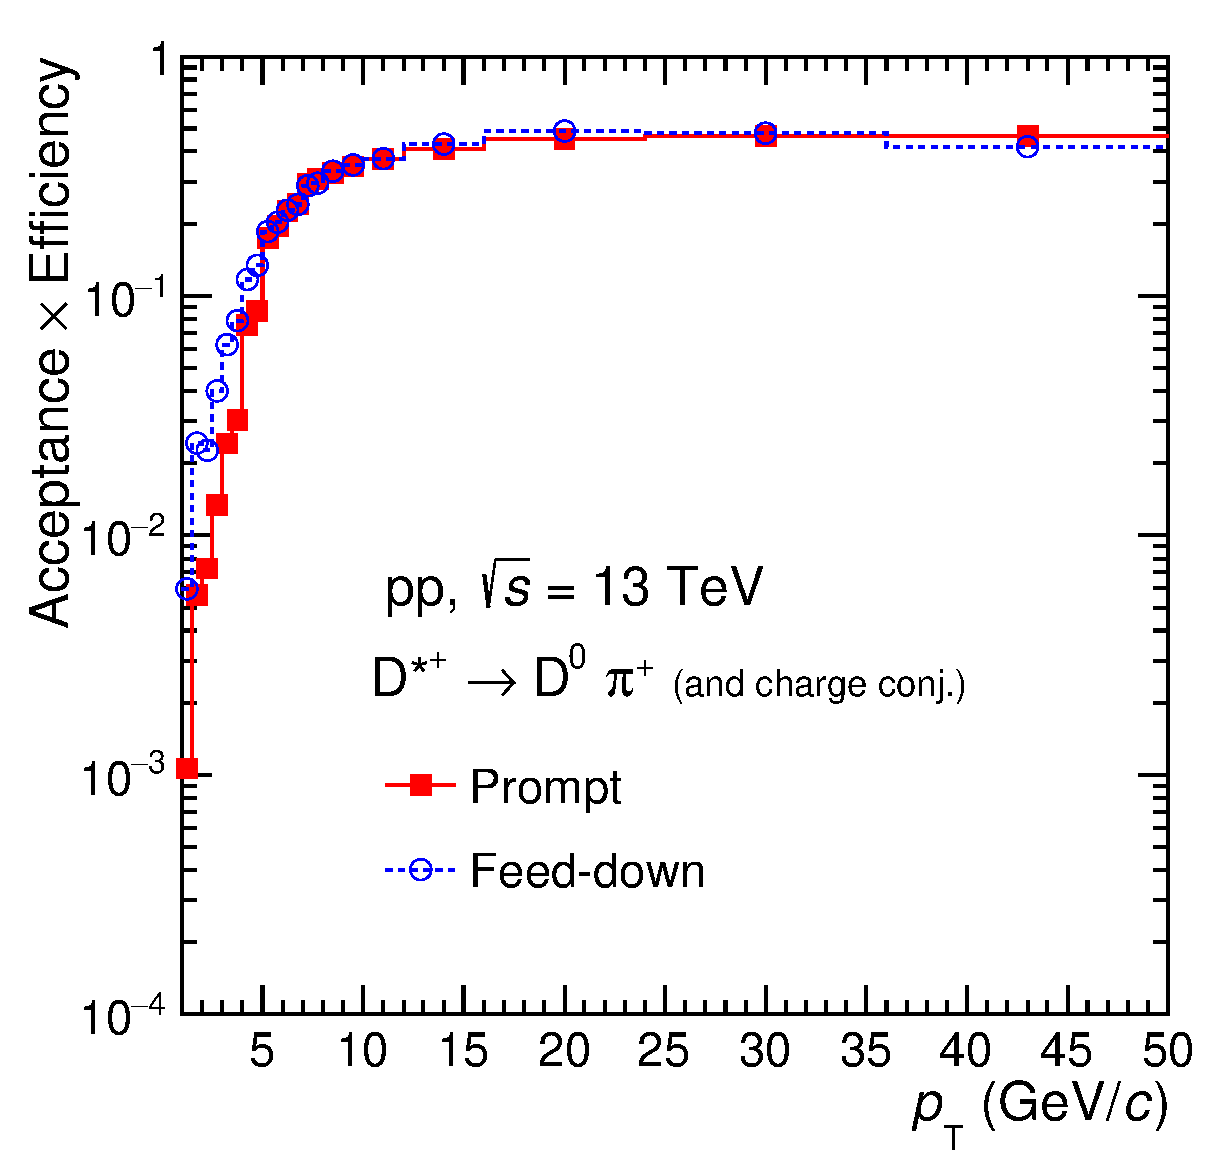
\includegraphics[width=0.8\textwidth]{figures/Dstar/pp13TeV/DstarAccEffVsPt_pp_13TeV.eps}
\caption{Transverse momentum dependence of efficiency$\times$acceptance for prompt (black) and feed-down (red).}
\label{fig:Dstar_eff}
\end{center}
\end{figure}
% Dplus efficiency


%\clearpage
\clearpage
\section{Systematic uncertainties}

\subsection{Raw yield extraction}
\label{sec:raw_yield_syst}
Several sources of systematic errors were considered for the four D mesons. The systematic error on the yield extraction was determined by repeating the fitting procedure described in section \ref{sec:sign_extr} with a different mass range, different histogram bin widths and/or different fitting functions, and using a method based on bin counting after the subtraction of the background estimated from the fit of the side bands. For the \Dzero meson, the variations listed above are obtained considering the yields once the reflection contribution has been subtracted.

The systematic uncertainty on the \Dplus, \Dzero, \Dstar and \Dsubs raw yield extraction was evaluated in each \pt interval using a multiple trial approach. The fits to the invariant mass distributions were repeated several times varying:
\begin{itemize}
	\item i) the invariant-mass bin width;
	\item ii) lower limit of the fit;
	\item iii)  upper  limit  of  the  fit;
	\item iv) for \Dzero, \Dplus, and \Dsubs, the background fit function (3 cases: exponential, linear and second order polynomial);
\end{itemize}   
In addition, all the fits were repeated with the sigma of the Gaussian function fixed to the values obtained from the MC simulation and the mean of the Gaussian function to the PDG value of the considered D-meson species mass. The fits which did not converge or had $\chi^2$/$ndf> $ 2.0 were rejected and not considered in the evaluation of the systematic uncertainty.  In addition, the results obtained with the fitting technique were compared to those obtained by counting the entries in the invariant mass histogram after subtracting the background counts calculated from the background fit function. Also for this check, a multiple trial approach was used. 
The results for \Dplus are shown in Figs. XX and YY, for the \Dzero in Figs. XX and YY, for \Dstar in Figs. XX and YY, and for \Dsubs in Figs.~\ref{fig:DsYieldSyst010_1},~\ref{fig:DsYieldSyst010_2} and YY.
For the \Dzero mesons the reflections subtraction procedure does not show a systematic effect, thus there is no need to assign a systematic uncertainty, as already shown in \cite{Bruna:2016mgn}. For the systematic uncertainty we took it almost from the rms of fit results. If the central raw yield between the mean of fit and bin counting doesn't differ, we do not consider the effect of shift; if not, we add in quadrature to the rms the maximum difference between the central value and the mean of the fits or of the bin counting.



\begin{figure}[!h]
\begin{center}
\includegraphics[width=0.7\textwidth]{figures/Dstar/pp13TeV/multi_trial/Mass_Spectra_stdBkg_1-4GeV.png} 
\includegraphics[width=0.7\textwidth]{figures/Dstar/pp13TeV/multi_trial/Mass_Spectra_stdBkg_4-7GeV.png}
\includegraphics[width=0.7\textwidth]{figures/Dstar/pp13TeV/multi_trial/Mass_Spectra_stdBkg_7-16GeV.png}
\includegraphics[width=0.7\textwidth]{figures/Dstar/pp13TeV/multi_trial/Mass_Spectra_stdBkg_16-50GeV.png} 
%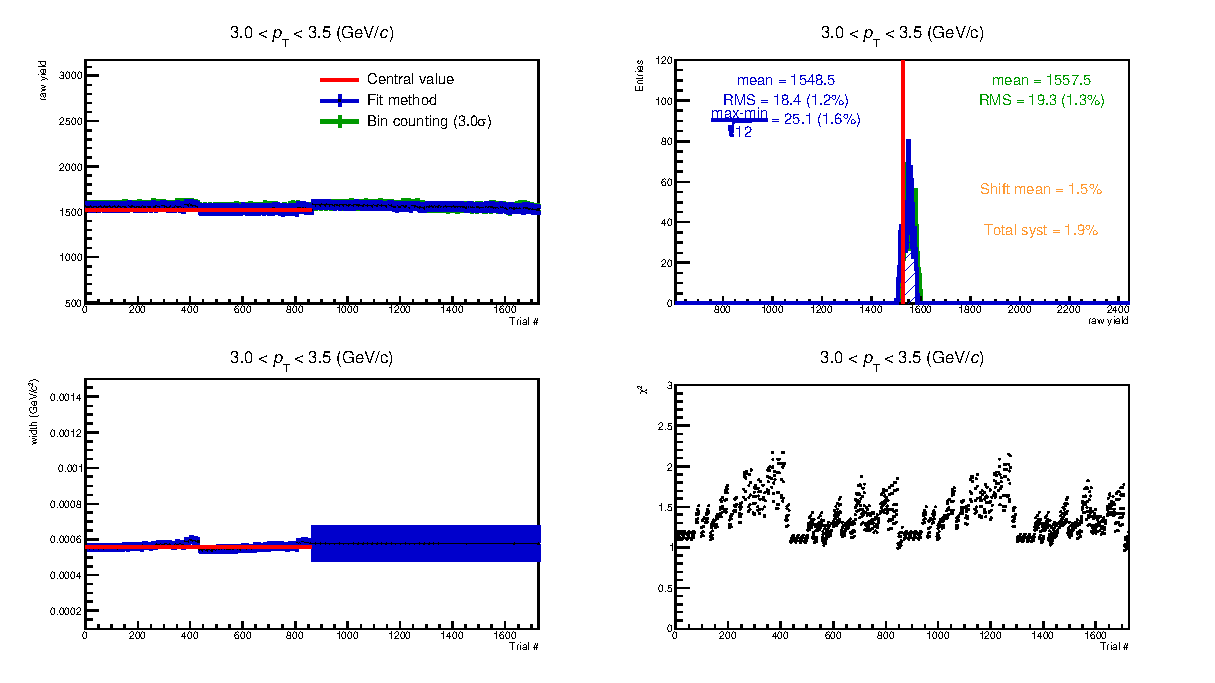
\includegraphics[width=0.8\textwidth]{figures/Dstar/pp13TeV/multi_trial/MultiFit_bkg5_3-3.eps}
%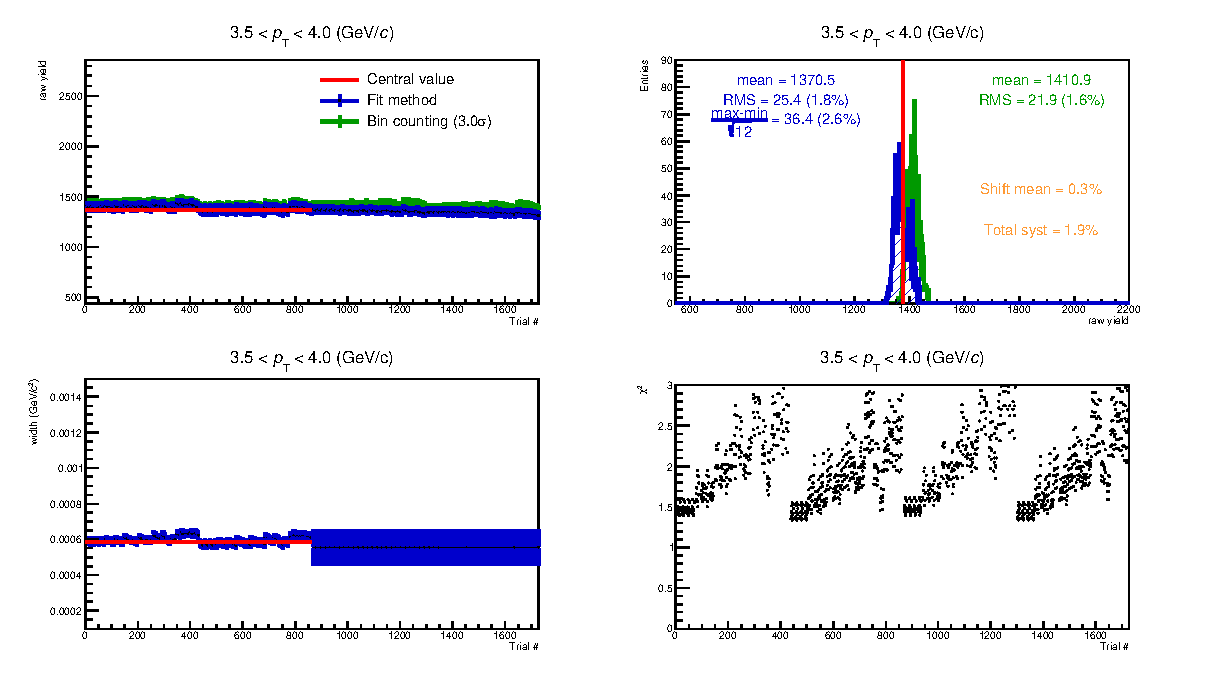
\includegraphics[width=0.65\textwidth]{figures/Dstar/pp13TeV/multi_trial/MultiFit_bkg5_3-4.eps}
%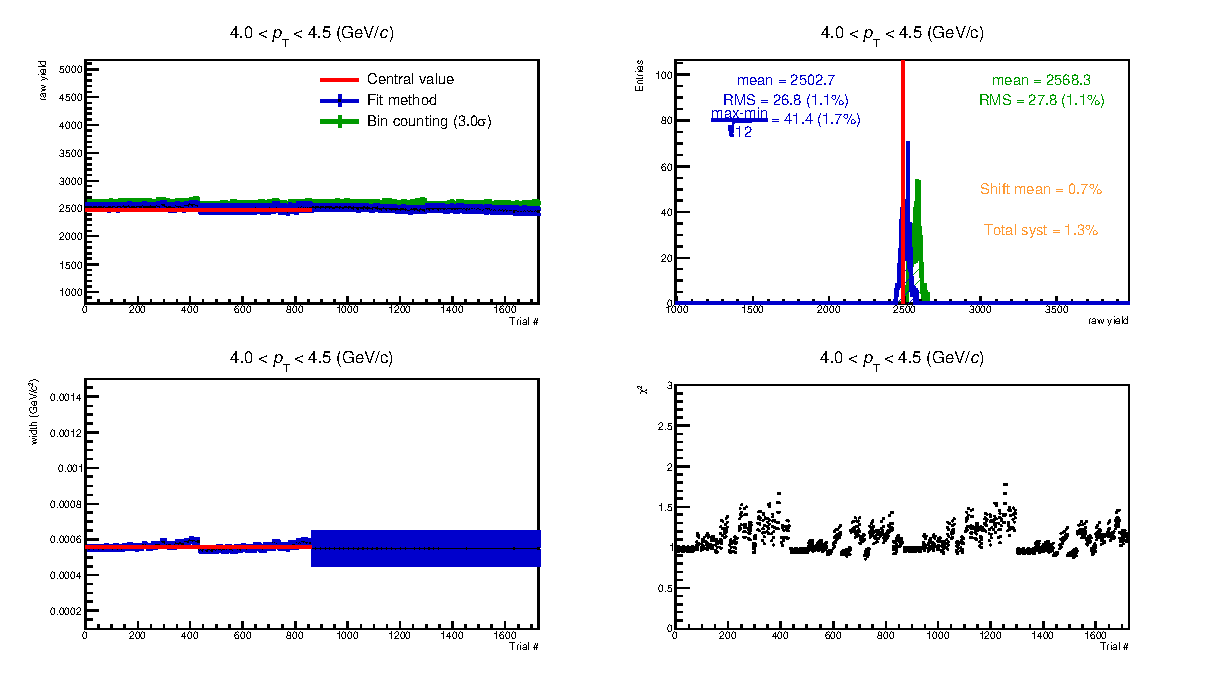
\includegraphics[width=0.65\textwidth]{figures/Dstar/pp13TeV/multi_trial/MultiFit_bkg5_4-4.eps}
\caption{\Dstar signal extraction using standard background fit function.}
\label{fig:DstarYield_stdbkg}
\end{center}
\end{figure}


\begin{figure}[!h]
\begin{center}
\includegraphics[width=0.3\textwidth]{figures/Dstar/pp13TeV/multi_trial/residual_plot_std_bkg_func_1-1dot5GeV.png} 
\includegraphics[width=0.3\textwidth]{figures/Dstar/pp13TeV/multi_trial/residual_plot_std_bkg_func_1dot5-2GeV.png}
\includegraphics[width=0.3\textwidth]{figures/Dstar/pp13TeV/multi_trial/residual_plot_std_bkg_func_2-2dot5GeV.png} 

\includegraphics[width=0.3\textwidth]{figures/Dstar/pp13TeV/multi_trial/residual_plot_stdBkg_func_2dot5-3GeV.png} 
\includegraphics[width=0.3\textwidth]{figures/Dstar/pp13TeV/multi_trial/residual_plot_std_bkg_func_3-3dot5GeV.png}
\includegraphics[width=0.3\textwidth]{figures/Dstar/pp13TeV/multi_trial/residual_plot_std_bkg_func_3dot5-4GeV.png} 

\includegraphics[width=0.3\textwidth]{figures/Dstar/pp13TeV/multi_trial/residual_plot_std_bkg_func_4-4dot5GeV.png} 
\includegraphics[width=0.3\textwidth]{figures/Dstar/pp13TeV/multi_trial/residual_plot_std_bkg_func_4dot5-5GeV.png}
\includegraphics[width=0.3\textwidth]{figures/Dstar/pp13TeV/multi_trial/residual_plot_std_bkg_func_5-5dot5GeV.png} 

\includegraphics[width=0.3\textwidth]{figures/Dstar/pp13TeV/multi_trial/residual_plot_std_bkg_func_5dot5-6GeV.png} 
\includegraphics[width=0.3\textwidth]{figures/Dstar/pp13TeV/multi_trial/residual_plot_std_bkg_func_6-6dot5GeV.png}
\includegraphics[width=0.3\textwidth]{figures/Dstar/pp13TeV/multi_trial/residual_plot_std_bkg_func_6dot5-7GeV.png} 

\includegraphics[width=0.3\textwidth]{figures/Dstar/pp13TeV/multi_trial/residual_plot_std_bkg_func_7-7dot5GeV.png} 
\includegraphics[width=0.3\textwidth]{figures/Dstar/pp13TeV/multi_trial/residual_plot_std_bkg_func_7dot5-8GeV.png}
\includegraphics[width=0.3\textwidth]{figures/Dstar/pp13TeV/multi_trial/residual_plot_std_bkg_func_8-9GeV.png} 

\includegraphics[width=0.3\textwidth]{figures/Dstar/pp13TeV/multi_trial/residual_plot_std_bkg_func_9-10GeV.png} 
\includegraphics[width=0.3\textwidth]{figures/Dstar/pp13TeV/multi_trial/residual_plot_std_bkg_func_10-12GeV.png}
\includegraphics[width=0.3\textwidth]{figures/Dstar/pp13TeV/multi_trial/residual_plot_std_bkg_func_12-16GeV.png} 

\includegraphics[width=0.3\textwidth]{figures/Dstar/pp13TeV/multi_trial/residual_plot_std_bkg_func_16-24GeV.png} 
\includegraphics[width=0.3\textwidth]{figures/Dstar/pp13TeV/multi_trial/residual_plot_std_bkg_func_24-36GeV.png}
\includegraphics[width=0.3\textwidth]{figures/Dstar/pp13TeV/multi_trial/residual_plot_std_bkg_func_36-50GeV.png} 

\caption{Residual plots using standard background fit function.}
\label{fig:DstarYield_stdbkg_residual}
\end{center}
\end{figure}


\begin{figure}[!h]
\begin{center}
\includegraphics[width=0.7\textwidth]{figures/Dstar/pp13TeV/multi_trial/Mass_Spectra_PowerFuncBkg_1-4GeV.png} 
\includegraphics[width=0.7\textwidth]{figures/Dstar/pp13TeV/multi_trial/Mass_Spectra_PowerFuncBkg_4-7GeV.png}
\includegraphics[width=0.7\textwidth]{figures/Dstar/pp13TeV/multi_trial/Mass_Spectra_PowerFuncBkg_7-16GeV.png}
\includegraphics[width=0.7\textwidth]{figures/Dstar/pp13TeV/multi_trial/Mass_Spectra_PowerFuncBkg_16-50GeV.png} 
%\includegraphics[width=0.8\textwidth]{figures/Dstar/pp13TeV/multi_trial/MultiFit_bkg5_3-3.eps}
%\includegraphics[width=0.65\textwidth]{figures/Dstar/pp13TeV/multi_trial/MultiFit_bkg5_3-4.eps}
%\includegraphics[width=0.65\textwidth]{figures/Dstar/pp13TeV/multi_trial/MultiFit_bkg5_4-4.eps}
\caption{\Dstar signal extraction using Power fit function for background.}
\label{fig:DstarYield_Powerbkg}
\end{center}
\end{figure}

\begin{figure}[!h]
\begin{center}
\includegraphics[width=0.3\textwidth]{figures/Dstar/pp13TeV/multi_trial/residual_plot_Pow_bkg_func_1-1dot5GeV.png} 
\includegraphics[width=0.3\textwidth]{figures/Dstar/pp13TeV/multi_trial/residual_plot_Pow_bkg_func_1dot5-2GeV.png}
\includegraphics[width=0.3\textwidth]{figures/Dstar/pp13TeV/multi_trial/residual_plot_Pow_bkg_func_2-2dot5GeV.png} 

\includegraphics[width=0.3\textwidth]{figures/Dstar/pp13TeV/multi_trial/residual_plot_Pow_bkg_func_2dot5-3GeV.png} 
\includegraphics[width=0.3\textwidth]{figures/Dstar/pp13TeV/multi_trial/residual_plot_Pow_bkg_func_3-3dot5GeV.png}
\includegraphics[width=0.3\textwidth]{figures/Dstar/pp13TeV/multi_trial/residual_plot_Pow_bkg_func_3dot5-4GeV.png} 

\includegraphics[width=0.3\textwidth]{figures/Dstar/pp13TeV/multi_trial/residual_plot_Pow_bkg_func_4-4dot5GeV.png} 
\includegraphics[width=0.3\textwidth]{figures/Dstar/pp13TeV/multi_trial/residual_plot_Pow_bkg_func_4dot5-5GeV.png}
\includegraphics[width=0.3\textwidth]{figures/Dstar/pp13TeV/multi_trial/residual_plot_Pow_bkg_func_5-5dot5GeV.png} 

\includegraphics[width=0.3\textwidth]{figures/Dstar/pp13TeV/multi_trial/residual_plot_Pow_bkg_func_5dot5-6GeV.png} 
\includegraphics[width=0.3\textwidth]{figures/Dstar/pp13TeV/multi_trial/residual_plot_Pow_bkg_func_6-6dot5GeV.png}
\includegraphics[width=0.3\textwidth]{figures/Dstar/pp13TeV/multi_trial/residual_plot_Pow_bkg_func_6dot5-7GeV.png} 

\includegraphics[width=0.3\textwidth]{figures/Dstar/pp13TeV/multi_trial/residual_plot_Pow_bkg_func_7-7dot5GeV.png} 
\includegraphics[width=0.3\textwidth]{figures/Dstar/pp13TeV/multi_trial/residual_plot_Pow_bkg_func_7dot5-8GeV.png}
\includegraphics[width=0.3\textwidth]{figures/Dstar/pp13TeV/multi_trial/residual_plot_Pow_bkg_func_8-9GeV.png} 

\includegraphics[width=0.3\textwidth]{figures/Dstar/pp13TeV/multi_trial/residual_plot_Pow_bkg_func_9-10GeV.png} 
\includegraphics[width=0.3\textwidth]{figures/Dstar/pp13TeV/multi_trial/residual_plot_Pow_bkg_func_10-12GeV.png}
\includegraphics[width=0.3\textwidth]{figures/Dstar/pp13TeV/multi_trial/residual_plot_Pow_bkg_func_12-16GeV.png} 

\includegraphics[width=0.3\textwidth]{figures/Dstar/pp13TeV/multi_trial/residual_plot_Pow_bkg_func_16-24GeV.png} 
\includegraphics[width=0.3\textwidth]{figures/Dstar/pp13TeV/multi_trial/residual_plot_Pow_bkg_func_24-36GeV.png}
\includegraphics[width=0.3\textwidth]{figures/Dstar/pp13TeV/multi_trial/residual_plot_Pow_bkg_func_36-50GeV.png} 

\caption{Residual plots using Power fit function for background.}
\label{fig:DstarYield_residual_power}
\end{center}
\end{figure}






%======= Dstar 0-10======= multi-trial ===========

\begin{figure}[!h]
\begin{center}
\includegraphics[width=0.68\textwidth]{figures/Dstar/pp13TeV/multi_trial/MultiFit_bkg4-Okt24_1-1.eps} 
\includegraphics[width=0.68\textwidth]{figures/Dstar/pp13TeV/multi_trial/MultiFit_bkg5-Okt24_1-2.eps}
\includegraphics[width=0.68\textwidth]{figures/Dstar/pp13TeV/multi_trial/MultiFit_bkg4-24Okt_2-2.eps}
\includegraphics[width=0.68\textwidth]{figures/Dstar/pp13TeV/multi_trial/MultiFit_bkg5_2-3.eps} 
%\includegraphics[width=0.8\textwidth]{figures/Dstar/pp13TeV/multi_trial/MultiFit_bkg5_3-3.eps}
%\includegraphics[width=0.65\textwidth]{figures/Dstar/pp13TeV/multi_trial/MultiFit_bkg5_3-4.eps}
%\includegraphics[width=0.65\textwidth]{figures/Dstar/pp13TeV/multi_trial/MultiFit_bkg5_4-4.eps}
\caption{Output of the multi-trial study for \Dstar mesons for $1<$ \pt$<3$ $\GeV/c$. For each \pt bin: the top panel shows the raw yield as a function of trials and raw yield distributions, the bottom panel shows the width and $\chi^2$ as a function of trials.}
\label{fig:DstarYieldSyst010_1}
\end{center}
\end{figure}


\begin{figure}[!h]
\begin{center}
\includegraphics[width=0.68\textwidth]{figures/Dstar/pp13TeV/multi_trial/MultiFit_bkg5_3-3.eps}
\includegraphics[width=0.68\textwidth]{figures/Dstar/pp13TeV/multi_trial/MultiFit_bkg5_3-4.eps}
\includegraphics[width=0.68\textwidth]{figures/Dstar/pp13TeV/multi_trial/MultiFit_bkg5_4-4.eps}
\includegraphics[width=0.68\textwidth]{figures/Dstar/pp13TeV/multi_trial/MultiFit_bkg5_4-5.eps}
\caption{Output of the multi-trial study for \Dstar mesons for $3<$ \pt$<5$ $\GeV/c$. For each \pt bin: the top panel shows the raw yield as a function of trials and raw yield distributions, the bottom panel shows the width and $\chi^2$ as a function of trials.}
\label{fig:DstarYieldSyst010_2}
\end{center}
\end{figure}

\begin{figure}[!h]
\begin{center}
\includegraphics[width=0.68\textwidth]{figures/Dstar/pp13TeV/multi_trial/MultiFit_bkg5_5-5.eps}
\includegraphics[width=0.68\textwidth]{figures/Dstar/pp13TeV/multi_trial/MultiFit_bkg5_5-6.eps}
\includegraphics[width=0.68\textwidth]{figures/Dstar/pp13TeV/multi_trial/MultiFit_bkg5_6-6.eps}
\includegraphics[width=0.68\textwidth]{figures/Dstar/pp13TeV/multi_trial/MultiFit_bkg5_6-7.eps}
\caption{Output of the multi-trial study for \Dstar mesons for $5<$ \pt$<7$ $\GeV/c$. For each \pt bin: the top panel shows the raw yield as a function of trials and raw yield distributions, the bottom panel shows the width and $\chi^2$ as a function of trials.}
\label{fig:DstarYieldSyst010_3}
\end{center}
\end{figure}


\begin{figure}[!h]
\begin{center}
\includegraphics[width=0.68\textwidth]{figures/Dstar/pp13TeV/multi_trial/MultiFit_bkg5_7-7.eps}
\includegraphics[width=0.68\textwidth]{figures/Dstar/pp13TeV/multi_trial/MultiFit_bkg5_7-8.eps}
\includegraphics[width=0.68\textwidth]{figures/Dstar/pp13TeV/multi_trial/MultiFit_bkg5_8-9.eps}
\includegraphics[width=0.68\textwidth]{figures/Dstar/pp13TeV/multi_trial/MultiFit_bkg5_9-10.eps}
\caption{Output of the multi-trial study for \Dstar mesons for $7<$ \pt$<10$ $\GeV/c$. For each \pt bin: the top panel shows the raw yield as a function of trials and raw yield distributions, the bottom panel shows the width and $\chi^2$ as a function of trials.}
\label{fig:DstarYieldSyst010_3}
\end{center}
\end{figure}



\begin{figure}[!h]
\begin{center}
\includegraphics[width=0.6\textwidth]{figures/Dstar/pp13TeV/multi_trial/MultiFit_bkg5_10-12.eps}
\includegraphics[width=0.6\textwidth]{figures/Dstar/pp13TeV/multi_trial/MultiFit_bkg5_12-16.eps}
\includegraphics[width=0.6\textwidth]{figures/Dstar/pp13TeV/multi_trial/MultiFit_bkg5_16-24.eps}
\includegraphics[width=0.5\textwidth]{figures/Dstar/pp13TeV/multi_trial/MultiFit_bkg5_24-36.eps}
\includegraphics[width=0.5\textwidth]{figures/Dstar/pp13TeV/multi_trial/MultiFit_bkg5_36-50.eps}
\caption{Output of the multi-trial study for \Dstar mesons for $10<$ \pt$<50$ $\GeV/c$. For each \pt bin: the top panel shows the raw yield as a function of trials and raw yield distributions, the bottom panel shows the width and $\chi^2$ as a function of trials.}
%\label{fig:DstarYieldSyst010_3}
\end{center}
\end{figure}



\begin{figure}[!h]
\begin{center}
\includegraphics[width=0.7\textwidth]{figures/Dstar/pp13TeV/multi_trial/multi_bin_bkg4alt_1-1dot5GeV.png}
\includegraphics[width=0.7\textwidth]{figures/Dstar/pp13TeV/multi_trial/multi_bin_bkg4std_1-1dot5GeV.png}
\includegraphics[width=0.7\textwidth]{figures/Dstar/pp13TeV/multi_trial/multi_bin_bkg5alt_1dot5-2GeV.png}
\includegraphics[width=0.7\textwidth]{figures/Dstar/pp13TeV/multi_trial/multi_bin_bkg5std_1dot5-2GeV.png}
%\includegraphics[width=0.5\textwidth]{figures/Dstar/pp13TeV/multi_trial/MultiFit_bkg5_36-50.eps}
\caption{Yield extration for \pt 1-2 GeV/$c$ tested with only one background function.}
%\label{fig:DstarYieldSyst010_3}
\end{center}
\end{figure}



%======= Dstar 0-10======= multi-trial ===========


The numerical values of the systematic on yield extraction, determined bin by bin for all the three non-strange D mesons are reported in Tables~\ref{tab:D0DplusDstarYieldSyst010} and ~\ref{tab:D0DplusDstarYieldSyst3050} and in Tables~\ref{tab:DsYieldSyst010} and~\ref{tab:DsYieldSyst3050} for \Dsubs.

\begin{table}[htbp]
 \begin{center}
  \begin{tabular}{|c|c|c|c|}
\hline
\pt ($\GeV/c$) &  \Dzero & \Dplus & \Dstar \\
\hline
1.0-1.5 & X & - & -\\
\hline
1.5-2.0 & X & - & -\\
\hline
2.0-2.5 & X & - & -\\
\hline
2.5-3.0 & X & 0.05 & -\\
\hline
3.0-3.5 & X & 0.05 & 0.06\\
\hline
3.5-4.0 & X & 0.05 & 0.04\\
\hline
4.0-4.5 & X & 0.05 & 0.04\\
\hline
4.5-5.0 & X & 0.05 & 0.04\\
\hline
5.0-5.5 & X & 0.05 & 0.04\\
\hline
5.5-6.0 & X & 0.05 & 0.04\\
\hline
6.0-6.5 & X & 0.05 & 0.04\\
\hline
6.5-7.0 & X & 0.05 & 0.04\\
\hline
7.0-7.5 & X & 0.05 & 0.03\\
\hline
7.5-8.0 & X & 0.05 & 0.03\\
\hline
8.0-9.0 & X & 0.05 & 0.03\\
\hline
9.0-10.0 & X & 0.03 & 0.03\\
\hline
10.0-12.0 & X & 0.03 & 0.03\\
\hline
12.0-16.0 & X & 0.03 & 0.03\\
\hline
16.0-24.0 & X & 0.03 & 0.03\\
\hline
24.0-36.0 & X & 0.03 & 0.03\\
\hline
36.0-50.0 & X & 0.05 & 0.03\\
\hline
  \end{tabular}
 \end{center}
 \caption{Systematic uncertainty from yield extraction for the \Dzero, \Dplus and \Dstar mesons in the 0--10\% centrality class.}
 \label{tab:D0DplusDstarYieldSyst010}
\end{table} 

\begin{table}[htbp]
 \begin{center}
  \begin{tabular}{|c|c|}
\hline
\pt ($\GeV/c$) &  \Dsubs \\
\hline
3.0-4.0 & 8\%\\
\hline
4.0-5.0 & 8\%\\
\hline
5.0-6.0 & 5\%\\
\hline
6.0-8.0 & 5\%\\
\hline
8.0-12.0 & 3\%\\
\hline
12.0-16.0 & 3\%\\
\hline
16.0-24.0 & 5\%\\
\hline
24.0-36.0 & 5\%\\
\hline
  \end{tabular}
 \end{center}
 \caption{Systematic uncertainty from yield extraction for the \Dsubs mesons in the 0--10\% centrality class.}
 \label{tab:DsYieldSyst010}
\end{table} 

\begin{table}[htbp]
 \begin{center}
  \begin{tabular}{|c|c|c|c|}
\hline
\pt ($\GeV/c$) &  \Dzero & \Dplus & \Dstar \\
\hline
1.0-1.5 & X & - & -\\
\hline
1.5-2.0 & X & - & -\\
\hline
2.0-2.5 & X & 0.07 & 0.05\\
\hline
2.5-3.0 & X & 0.07 & 0.05\\
\hline
3.0-3.5 & X & 0.04 & 0.05\\
\hline
3.5-4.0 & X & 0.04 & 0.03\\
\hline
4.0-4.5 & X & 0.04 & 0.03\\
\hline
4.5-5.0 & X & 0.03 & 0.03\\
\hline
5.0-5.5 & X & 0.03 & 0.03\\
\hline
5.5-6.0 & X & 0.03 & 0.03\\
\hline
6.0-6.5 & X & 0.03 & 0.03\\
\hline
6.5-7.0 & X & 0.03 & 0.03\\
\hline
7.0-7.5 & X & 0.03 & 0.03\\
\hline
7.5-8.0 & X & 0.03 & 0.03\\
\hline
8.0-9.0 & X & 0.03 & 0.03\\
\hline
9.0-10.0 & X & 0.03 & 0.03\\
\hline
10.0-12.0 & X & 0.03 & 0.03\\
\hline
12.0-16.0 & X & 0.03 & 0.03\\
\hline
16.0-24.0 & X & 0.04 & 0.03\\
\hline
24.0-36.0 & X & 0.06 & 0.03\\
\hline
36.0-50.0 & X & 0.08 & -\\
\hline
  \end{tabular}
 \end{center}
 \caption{Systematic uncertainty from yield extraction for the \Dzero, \Dplus and \Dstar mesons in the 30--50\% centrality class.}
 \label{tab:D0DplusDstarYieldSyst3050}
\end{table} 

\begin{table}[htbp]
 \begin{center}
  \begin{tabular}{|c|c|}
\hline
\pt ($\GeV/c$) &  \Dsubs \\
\hline
3.0-4.0 & 9\%\\
\hline
4.0-6.0 & 6\%\\
\hline
6.0-8.0 & 4\%\\
\hline
8.0-12.0 & 4\%\\
\hline
12.0-16.0 & 2\%\\
\hline
16.0-24.0 & 3\%\\
\hline
  \end{tabular}
 \end{center}
 \caption{Systematic uncertainty from yield extraction for the \Dsubs mesons in the 30--50\% centrality class.}
 \label{tab:DsYieldSyst3050}
\end{table} 


%#######################################################################
\clearpage
\subsection{Selection efficiency}
\label{sec:eff_syst}
A further systematic uncertainty can arise from possible differences in the cut-variable
shapes in data and Monte Carlo and due to residual misalignment. This
sources where checked by repeating the analysis varying the
selection cuts from the standard set of
cuts. Moving the main cuts all left or all right may introduce a bias
due to the fact that all the cuts goes in the same direction. Due to
this concern, different sets of cuts, alternative to the standard one were tested. 

For the \Dsubs meson, a systematic scan from loose to tight cuts was done on a variable
per variable basis, reconstructing the yields, comparing them to the yields obtained with a reference set of
cuts and looking for possible trends/biases of the reconstructed yield as a function of the cut strength. The result of this study for each \pt bin is shown n Figs.~\ref{fig:DsCutSyst010_1} and~\ref{fig:DsCutSyst010_1}, where the variations of the raw yield, prompt and feed-down \Dsubs efficiency, significance, signal-to-background ratio, and corrected yield are plotted as a function of the cut set tested. Finally the distribution of the variation of the corrected yield is shown. All the trials for which the extracted yield had a significance larger than 3 and a variation of the efficiency larger than 1\% were taken into account. The systematic uncertainty was assigned considering the rms and the deviation from unity of these distributions. The values are reported in Table~\ref{tab:DsCutSyst010}. 

For the \Dstar meson, a systematic scan from loose to tight cuts was done by varying the variables: dca, d0$\times$d0, \pt kaon and \pt pion. The result of this study is shown in Figs.~\ref{fig:DstarCutVar010} and ~\ref{fig:DstarCutVar3050}, where the variation of the rawyield, prompt efficiency, and corrected yield ratio are plotted as a function of the cut set tested.

For the \Dplus meson, a systematic scan from loose to tight cuts was done by varying the variables. The result of this study is shown in Figs.~\ref{fig:DplusCutVar010} and ~\ref{fig:DplusCutVar3050}, where the variation of the rawyield, prompt efficiency, and corrected yield ratio are plotted as a function of the cut set tested.



\begin{table}[htbp]
 \begin{center}
  \begin{tabular}{|c|c|c|c|}
\hline
\pt ($\GeV/c$) &  \Dzero & \Dplus & \Dstar \\
\hline
1.0-1.5 & X & - & -\\
\hline
1.5-2.0 & X & - & -\\
\hline
2.0-2.5 & X & - & -\\
\hline
2.5-3.0 & X & 10 & -\\
\hline
3.0-3.5 & X & 6 & 12\% \\
\hline
3.5-4.0 & X & 6 & 10\% \\
\hline
4.0-4.5 & X & 6 & 10\% \\
\hline
4.5-5.0 & X & 6 & 10\% \\
\hline
5.0-5.5 & X & 6 & 8\% \\
\hline
5.5-6.0 & X & 5 & 8\% \\
\hline
6.0-6.5 & X & 5 & 8\% \\
\hline
6.5-7.0 & X & 4 & 8\% \\
\hline
7.0-7.5 & X & 4 & 8\% \\
\hline
7.5-8.0 & X & 4 & 8\% \\
\hline
8.0-9.0 & X & 3 & 8\% \\
\hline
9.0-10.0 & X & 3 & 8\% \\
\hline
10.0-12.0 & X & 3 & 6\% \\
\hline
12.0-16.0 & X & 3 & 4\% \\
\hline
16.0-24.0 & X & 3 & 4\% \\
\hline
24.0-36.0 & X & 4 & 4\%\\
\hline
36.0-50.0 & X & 4 & 2\% \\
\hline
  \end{tabular}
 \end{center}
 \caption{Systematic uncertainty estimated with the cut-variation study for the \Dzero, \Dplus, and \Dstar mesons in the 0--10\% centrality class.}
 \label{tab:D0DplusDstarCutSyst010}
\end{table} 


\begin{table}[htbp]
 \begin{center}
  \begin{tabular}{|c|c|c|c|}
\hline
\pt ($\GeV/c$) &  \Dzero & \Dplus & \Dstar \\
\hline
1.0-1.5 & X & - & -\\
\hline
1.5-2.0 & X & - & -\\
\hline
2.0-2.5 & X & 7 & 18\% \\
\hline
2.5-3.0 & X & 5 & 6\% \\
\hline
3.0-3.5 & X & 5 & 6\% \\
\hline
3.5-4.0 & X & 4 & 6\% \\
\hline
4.0-4.5 & X & 4 & 6\% \\
\hline
4.5-5.0 & X & 4 & 6\% \\
\hline
5.0-5.5 & X & 4 & 6\% \\
\hline
5.5-6.0 & X & 4 & 6\% \\
\hline
6.0-6.5 & X & 2 & 6\% \\
\hline
6.5-7.0 & X & 2 & 6\% \\
\hline
7.0-7.5 & X & 2 & 6\% \\
\hline
7.5-8.0 & X & 2 & 6\% \\
\hline
8.0-9.0 & X & 2 & 6\% \\
\hline
9.0-10.0 & X & 2 & 2\% \\
\hline
10.0-12.0 & X & 2 & 0 \\
\hline
12.0-16.0 & X & 2 & 0 \\
\hline
16.0-24.0 & X & 2 & 0 \\
\hline
24.0-36.0 & X & 4 & 0 \\
\hline
36.0-50.0 & X & 6 & -\\
\hline
  \end{tabular}
 \end{center}
 \caption{Systematic uncertainty estimated with the cut-variation study for the \Dzero, \Dplus, and \Dstar mesons in the 30--50\% centrality class.}
 \label{tab:D0DplusDstarCutSyst3050}
\end{table} 




%======= Dstar =======
\begin{figure}[tb]
\begin{center}
\includegraphics[width=0.8\textwidth]{figures/Dstar/pp13TeV/signal-cut-variation.pdf}
 \includegraphics[width=0.8\textwidth]{figures/Dstar/pp13TeV/signal-ratio-cut-variation.pdf}
 \includegraphics[width=0.8\textwidth]{figures/Dstar/pp13TeV/prompt-ratio-cut-variation.pdf} % signal_ratio_010cc_cutVariation.pdf
 \includegraphics[width=0.8\textwidth]{figures/Dstar/pp13TeV/corrected-yield-ratio-cut-var-v2.pdf}
\caption{Variations of raw yield, prompt  efficiency, and corrected yield obtained with the cut-variation study for the \Dstar mesons in the 0--10\% centrality class.}
\label{fig:DstarCutVar010}
\end{center}
\end{figure}


%=======================================================================
\clearpage
\subsection{Generated \pt shape}
\label{sec:gen_pt_syst}
Another source of systematic we investigated is the one arising from the D meson \pt shape assumed in the Monte Carlo used for corrections. In our simulation the D mesons are folded in the HIJING event using PYTHIA and as a result the \pt shape of the D mesons can be biased leading to an effect in the final efficiency used for corrections. In order to check the stability of our efficiencies against the change in \pt shape and to define a systematic uncertainty it was decided to implement several set of weights. 

For the \Dsubs meson, the \pt shapes provided by different models were taken into account. For the default value, the \pt shape of TAMU was considered, since it implements both the in-medium energy loss and the enhanced \Dsubs production due to the hadronisation via coalescence in a strange-rich medium. For the variation, the shapes of PHSD, Catania models, which also provide predictions for the \Dsubs mesons were considered. In addition, the MC@sHQ model for non-strange D mesons was considered to take into account a scenario in which the \Dsubs is not enhanced and as extreme case FONLL that assumes no suppression. 

The \pt shapes and the corresponding \pt weights, obtained by dividing each shape by the one of the MC simulation, are reported in Fig.~\ref{fig:DsPtWeights010} and Fig.~\ref{fig:DsPtWeights3050} for the 0--10\% and 30--50\% centrality classes. The variation of the efficiency of prompt \Dsubs mesons is reported in Fig.~\ref{fig:DsPtShapeSyst010} and Fig.~\ref{fig:DsPtShapeSyst3050}. For the 0--10\% centrality class, 2\% systematic was assigned in the range $3<$\pt$<12~\GeV/c$, while no systematic uncertainty was assigned for \pt$>12~\GeV/c$.
For the 30--50\% centrality class, 3\% systematic was assigned in the range $3<$\pt$<6~\GeV/c$, 1\%  in the range $8<$\pt$<12~\GeV/c$ while no systematic uncertainty was assigned for \pt$>12~\GeV/c$.

For the non-strange D mesons 0--10\% centrality class, the re-weighted shape was obtained from the mixture of the measured \Dzero corrected yield shape with FONLL predictions, used in \pt regions where the measurement is not feasible or not precise. Then, other \pt weight was considered to check the stability of the efficiencies against the \pt shape of the generated D mesons. For the 0--10\% centrality class, the systematic uncertainty was evaluated comparing the central values of the efficiency obtained using the FONLL times LBT. For the 30--50\% centrality class, the systematic uncertainty was evaluated comparing the central values of the efficiency (applying FONLL5andBAMPS weight) to that obtained applying the FONLL weight.


%======= Dstar =======
\begin{figure}[tb]
\begin{center}
 \includegraphics[width=0.8\textwidth]{figures/Dstar/pp13TeV/MCpTShape_syst.png}
 \includegraphics[width=0.95\textwidth]{figures/Dstar/pp13TeV/ratio-cross-section-MC-pT-shpae.pdf}
\caption{Relative change in efficiencies by using PYTHIA8 (central) with respect to FONLL5anddata (syatematic) weight.}
\label{fig:DstarPtWeights010}
\end{center}
\end{figure}
%======= Dstar =======



\begin{table}[htbp]
 \begin{center}
  \begin{tabular}{|c|c|c|c|}
\hline
\pt ($\GeV/c$) &  \Dzero & \Dplus & \Dstar \\
\hline
1.0-1.5 & X & - & -\\
\hline
1.5-2.0 & X & - & -\\
\hline
2.0-2.5 & X & - & -\\
\hline
2.5-3.0 & X & 2 & -\\
\hline
3.0-3.5 & X & 1 & 1\% \\
\hline
3.5-4.0 & X & 1 & 0.5\% \\
\hline
4.0-4.5 & X & 1 & 0\\
\hline
4.5-5.0 & X & 1 & 0\\
\hline
5.0-5.5 & X & 0 & 0\\
\hline
5.5-6.0 & X & 0 & 0\\
\hline
6.0-6.5 & X & 0 & 0\\
\hline
6.5-7.0 & X & 0 & 0\\
\hline
7.0-7.5 & X & 0 & 0\\
\hline
7.5-8.0 & X & 0 & 0\\
\hline
8.0-9.0 & X & 0 & 0\\
\hline
9.0-10.0 & X & 0 & 0\\
\hline
10.0-12.0 & X & 0 & 0\\
\hline
12.0-16.0 & X & 0 & 0\\
\hline
16.0-24.0 & X & 0 & 0\\
\hline
24.0-36.0 & X & 0 & 0\\
\hline
36.0-50.0 & X & 0 & -\\
\hline
  \end{tabular}
 \end{center}
 \caption{Systematic uncertainty estimated with the MC \pt shape study for the \Dzero, \Dplus, and \Dstar mesons in the 0--10\% centrality class.}
 \label{tab:D0DplusDstarMCpTshape010}
\end{table} 

\clearpage
\subsection{PID efficiency}
The systematic uncertainty on the PID selection efficiency was evaluated with a per-track study, using relatively pure samples of pions and kaons. Pions were selected from $\rm K_{\rm s}^0$ and $\Lambda$ decays, while kaons in the TPC (TOF) were selected applying a tight selection on the PID signal in the TOF (TPC) of $|N_{\sigma}(\rm K)|<0.2$.  

However, for this data sample, a discrepancy between the TPC PID efficiency in data and MC simulation up to 5\%, 15\%, 30\% for a $3\,\sigma$, $2\,\sigma$, and $1\,\sigma$ selection, respectively, was observed. This was caused by an imperfect calibration of the expected $\de E/\de x$ for the different hadron species in the data, which was reflected in a deviation of the $N_{\sigma}^{\rm TPC}$ distributions from the Normal distribution. In order to avoid large biases in the D-meson measurement, a post-calibration procedure was applied to correct the $N_{\sigma}^{\rm TPC}$ values. In particular, the distributions obtained from the pure samples of pions and kaons were fitted with a Gaussian function to extract the mean, $\langle N_{\sigma}^{\rm TPC}\rangle$, and the width, $\sigma(N_{\sigma}^{\rm TPC})$, of the uncalibrated distributions of pions and kaons. The extracted parameters were then used to compute the corrected $N_{\sigma}^{\rm TPC, corr}$ value for each track as
\begin{equation}
N_{\sigma}^{\rm TPC, corr} (X) = \frac{N_{\sigma}^{\rm TPC} (X)-\langle N_{\sigma}^{\rm TPC} (X) \rangle}{\sigma(N_{\sigma}^{\rm TPC} (X))},
\end{equation}
where $X$ stands for a given mass hypothesis, i.e. pion or kaon. This procedure was performed in intervals of track momentum and pseudorapidity. Figures~\ref{fig:NsigmaTPCuncorr18q} and~\ref{fig:NsigmaTPCuncorr18r} show the $N_{\sigma}^{\rm TPC}$ distributions as a function of pseudorapidity before the post calibration for the LHC18q and LHC18r periods, respectively, while Fig.~\ref{fig:NsigmaTPCcorr} after the post-calibration for both the periods for the 0--10\% centrality class. Samples of pions, kaons and protons independent of the one used to compute the correction were used to cross check the goodness of the post-calibration. The mean value of the distribution before the correction is shifted towards negative values, and shows a clear $\eta$-dependence. The corrected distribution is constantly centred at zero as a function of $\eta$. The residual deviation from unity in the kaon and proton distributions is due to residual contamination in the samples.

\begin{figure}[tb]
\begin{center}
\includegraphics[width=0.8\textwidth]{figures/Dstar/pp13TeV/rawyield_ratio_PID_noPID-new.pdf}
 \includegraphics[width=0.8\textwidth]{figures/Dstar/pp13TeV/prompt_PID_noPID_ratio-v3.pdf}
 \includegraphics[width=0.8\textwidth]{figures/Dstar/pp13TeV/cross-section-comaprison-PID-noPID.pdf}
 \includegraphics[width=0.8\textwidth]{figures/Dstar/pp13TeV/cross-section-ratio_PID_noPID-updated.pdf}
\caption{PID systematic \Dstar meson.}
\label{fig:NsigmaTPCuncorr18q}
\end{center}
\end{figure}


In Figs.~\ref{fig:effPionPID} and~\ref{fig:effKaonPID} the data-to-MC ratios of the $N_{\sigma}^{\rm TPC}$ and $N_{\sigma}^{\rm TOF}$ selection efficiencies of pions and kaons as a function of $\pt$ in the 0--10\% centrality class for a $3\,\sigma$, $2\,\sigma$, and $1\,\sigma$ selection after the TPC recalibration procedure. A similar result was obtained in the 30--50\% centrality class. The deviation from unity of these ratios was considered as systematic uncertainty on the single track. 


The single-track systematic uncertainty was propagated to the D mesons using the decay kinematics of the MC simulation used for the analysis. Figs.~\ref{fig:DsPIDsyst},~\ref{fig:DsPIDsystStrong} and~\ref{fig:DzeroPIDsyst} show the systematic uncertainty obtained for the \Dsubs and \Dzero mesons in the 0--10\% centrality class. The uncertainty for the conservative PID strategy was assigned to the \Dsubs-meson measurement for $\pt<8~\GeV/c$, while that for the strong PID strategy at higher $\pt$. 


\clearpage
\subsection{Track reconstruction efficiency}

The systematic uncertainty due to the track-reconstruction efficiency includes the contributions of the track-finding procedure in the TPC detector and prolongation in the ITS detector, and the track-quality selections. 

The ITS-TPC matching efficiency was computed as the number of tracks successfully fitted with the Kalman filter in the TPC and ITS, with at least one hit in the SPD layers, divided by the number of reconstructed tracks successfully fitted in the TPC. The systematic uncertainty on its determination arises from discrepancies in the tracking performance between data and the MC simulation. The ITS-TPC matching efficiency is different for particles produced in the collision, including strong decays and weak decays of charm and beauty hadrons, which are considered as primary particles in this study, and secondary particles (i.e. particles produced in the interactions with the material or in decays of strange hadrons). The HIJING event generator and the GEANT3 transport package do not reproduce the relative abundance of primary and secondary particles, therefore data-driven corrections for the fraction of primary particles ($f_{\rm primary}$) were used to weight the MC simulation and obtain the corrected inclusive MC efficiency ($\epsilon_{\rm inclusive}({\rm MC})$), which is computed as:
\begin{equation}
	\epsilon_{\rm inclusive}({\rm MC}) = f_{\rm primary}\cdot\epsilon_{\rm primary}({\rm MC})+(1-f_{\rm primary})\cdot\epsilon_{\rm secondary}({\rm MC}),
\end{equation}
where $\epsilon_{\rm primary}({\rm MC})$ and $\epsilon_{\rm secondary}({\rm MC})$ are the ITS-TPC matching efficiencies for primary and secondary particles, which are determined via fits to the $d_0^{xy}$ distributions of the tracks. 

In addition, it was checked if a discrepancy between the efficiency of the track-quality selections in data and in the MC simulation need to be considered. For this purpose, the D-meson cross section was re-evaluated with three alternative track-quality selection criteria, which include the selection of tracks with (i) a number TPC crossed rows larger than $120-5/(\pt~[\GeV/c])$ instead of the default value of 70, (ii)  the number of TPC clusters at least 0.65 times the number of TPC crossed rows and (iii) a ratio of crossed rows over findable clusters in the TPC larger than 0.9 (being the default 0.8). These variations are shown for the \Dsubs meson in the 0--10\% centrality class in Fig.~\ref{}.
The variation of the cross section was observed to be around 1.0\% for \Dzero (two-body decay) and 1.5\% for the other D mesons (three-body decays), therefore a value equal to 0.5\% was added to the per-track systematic uncertainty estimated for the ITS-TPC matching efficiency. 

\begin{figure}[tb]
\begin{center}
 \includegraphics[width=0.9\textwidth]{figures/Dstar/pp13TeV/corrected-yield-ratio-tracking-Dstar-D0-single-track.pdf}
 \includegraphics[width=0.9\textwidth]{figures/Dstar/pp13TeV/tracking-soft-pion-ratio-cross-section.pdf}
\caption{Comparison of \Dstar corrected yield measured obtained with different TPC track-quality criteria.}
\label{fig:TrackVariations}
\end{center}
\end{figure}

Finally, the $\pt$-dependent per-track systematic uncertainty was propagated to the \Dsubs mesons via the kinematics of the \Dsubs daughter tracks, similarly to the procedure explained in the previous Section for the PID uncertainty. The systematic uncertainties obtained for \Dsubs and \Dzero mesons in the 0--10\% centrality class are shown in Figs.~\ref{fig:DsTrackSyst} and~\ref{fig:DzeroTrackSyst}.


\begin{figure}[tb]
\begin{center}
 \includegraphics[width=0.9\textwidth]{figures/Dstar/pp13TeV/Dstar-ME-eff-final.pdf}
\caption{Systematic uncertainty on tracking efficiency assigned to \Dstar mesons.}
\label{fig:DzeroTrackSyst}
\end{center}
\end{figure}





%\clearpage
\section{Feed-down subtraction}
%The methods for B feed-down subtraction
%As described in Sec.~\ref{sec:eff}, the prompt D meson production yields ${\rmd}N/{\rm d}\pt$ in Pb--Pb 
%collisions were obtained by subtracting the contribution of D mesons from B decays with the same procedure used for the measurement of the production cross sections in pp collisions~\cite{Acharya:2019mgn}. In detail, 

The feed-down contribution was estimated using 
the beauty production cross section from the FONLL calculation,
the B$\rightarrow$D decay kinematics from the EvtGen package,
and the Monte Carlo efficiencies for feed-down D mesons. 
%For Pb--Pb collisions, 
%the FONLL feed-down cross section in pp at $\sqrt{s}=5.02~\TeV$ 
%was scaled by the average nuclear overlap function $\langle \TAA \rangle$ in
%each centrality class.
Thus, omitting for brevity the symbol of the $\pt$-dependence $(\pt)$, 
the fraction of prompt D mesons reads:
\begin{equation}
 \label{eq:fcNbMethod}
 \begin{split}
   f_{\rm prompt} &= 1-(N^{\rm D~feed-down~raw}/N^{\rm D~raw})\\
   &= 1 -  \left( \frac{{\rm d}^2 \sigma}{{\rm d}y \, {\rm d}\pt }
\right)^{{\sf FONLL}} _{{\rm feed-down}} \cdot
\frac{({\rm Acc}\times\epsilon)_{\rm feed-down}\cdot\Delta y \, \Delta\pt
\cdot {\rm BR} \cdot L_{\rm int}  }{ N^{\rm D~raw }  / 2} \, ,
 \end{split}
\end{equation}
where $({\rm Acc}\times\epsilon)_{{\rm feed-down}}$ is the 
acceptance-times-efficiency for feed-down D mesons and the factor 2 at the denominator
comes for counting both particle and antiparticle
are combined while in FONLL not. The nuclear modification factor of the feed-down D mesons, $\RAA^{\rm feed-down}$,
is related to the nuclear modification of beauty production in Pb--Pb 
collisions, which is currently unknown. Taking advantage of the
recent non-prompt J/$\Psi$ results from the CMS collaboration we
assumed for the correction that the nuclear modification factor 
for feed-down is equal to two times the one of the prompt D mesons ($\RAA^{\rm feed-down}=2\RAA^{\rm prompt}$) and varied this hypothesis
in the range $1<\RAA^{\rm feed-down}/\RAA^{\rm prompt}<3$ ($1/3<\RAA^{\rm feed-down}/\RAA^{\rm prompt}<3$ for \Dsubs)
to determine the systematic uncertainty. In the left panel of Fig. \ref{fig:Dsfeeddown010} (Fig. \ref{fig:Dsfeeddown3050})
the variation of $\RAA^{\rm prompt}$ for \Dsubs mesons in the 0--10\% (30--50\%) centrality class is shown as a function of
this hypothesis for some (all) $\pt$ intervals of the analysis. The resulting fraction of prompt \Dsubs in the same centrality class is reported in the right panel of the same figure.
In Fig.~\ref{fig:Dzerofeeddown_cent} and \ref{fig:Dzerofeeddown_semicent} the variation of $\RAA^{\rm prompt}$ for \Dzero mesons in the 0--10\% and 30-50\% centrality classes are reported as a function of this hypothesis for some \pt intervals of the analysis in the left panel of each figure. The resulting fraction of prompt \Dzero in the same centrality classes are reported as line histogram in the right panel of the Fig.~\ref{fig:Dzerofeeddown_cent} and \ref{fig:Dzerofeeddown_semicent}.
In addition, to estimate the systematic uncertainty, the perturbative uncertainty on the FONLL beauty production cross section was considered, by varying the b quark mass and the factorization and renormalization scales as suggested in~\cite{Acharya:2019mgn}. 



%======= Dstar =====
\begin{figure}[tb]
\begin{center}
 \includegraphics[width=0.9\textwidth]{figures/Dstar/pp13TeV/feed-down-syst-Dstar.pdf}
\caption{Fraction of prompt \Dstar estimated using the FONLL-based approach.}
\label{fig:Dstarfeeddown_cent}
\end{center}
\end{figure}




\begin{figure}[tb]
\begin{center}
 \includegraphics[width=1\textwidth]{figures/Dstar/pp13TeV/RelativeSystematics.eps}
\caption{Relative systematic uncertainties on the \pt -differential production cross
section of prompt \Dstar mesons.}
\label{fig:DstarSystSum}
\end{center}
\end{figure}

%\clearpage
\section{Results}
In this Section, the results obtained are reported. The corrected yields of the \Dstar is shown in Fig.~\ref{fig:DmesonCorrYields}. In Fig.~\ref{fig:DmesonCorrYieldsModel}, the $\pt$-differential cross section of prompt \Dstar is compared to theoretical model, FONLL.


\begin{figure}[tb]
\begin{center}
%\includegraphics[width=0.48\textwidth]{PlotsRAA/Dzero_dNdpt_010_3050.pdf}
%\includegraphics[width=0.48\textwidth]{PlotsRAA/Dplus_dNdpt_010_3050.pdf}
\includegraphics[width=0.65\textwidth]{figures/Dstar/pp13TeV/cross-setion-pp13TeV.png}
%\includegraphics[width=0.48\textwidth]{PlotsRAA/Ds_dNdpt_010_3050.pdf}
\caption{$\pt$-differential inclusive production cross section of prompt \Dstar mesons in pp collisions at \s 13 TeV.} 
% pT -differential inclusive production cross section of prompt
\label{fig:DmesonCorrYields}
\end{center}
\end{figure}



\begin{figure}[tb]
\begin{center}
%\includegraphics[width=0.48\textwidth]{PlotsRAA/Dzero_dNdpt_010_3050.pdf}
%\includegraphics[width=0.48\textwidth]{PlotsRAA/Dplus_dNdpt_010_3050.pdf}
\includegraphics[width=0.65\textwidth]{figures/Dstar/pp13TeV/comparison_plt_dstar.png}
%\includegraphics[width=0.48\textwidth]{PlotsRAA/Ds_dNdpt_010_3050.pdf}
\caption{Comparison new analysis full data sample (2016, 2017 and 2018) with respect to the only 2016 data in pp collisions at \s 13 TeV.} 
% pT -differential inclusive production cross section of prompt
\label{fig:DmesonCorrYields}
\end{center}
\end{figure}


\begin{figure}[tb]
\begin{center}
\includegraphics[width=1\textwidth]{figures/Dstar/pp13TeV/cross-section-pp13TeV-final-systematics.pdf}
\caption{$\pt$-differential inclusive production cross section of prompt \Dstar mesons in pp collisions at \s 13 TeV compared with FONLL.}
\label{fig:DmesonCorrYieldsModel}
\end{center}
\end{figure}

%\newpage
%\input{results.tex}


\clearpage
\bibliographystyle{utphys}
\bibliography{biblio.bib}
\end{document}
